\subsection{Complete evaluation and label effects}
All 320 assignments yielded complete programs and native outcomes, with no retry, missing result or evaluation timeout. Of the 316 control-eligible outcomes, 173 pass and 143 fail. The four outcomes on /59 remain visible in the complete task appendix (three passes and one failure), but do not enter quality inference. Table~\ref{tab:seg80-groups} gives the four condition totals.
\begin{table}[t]\centering\small
\caption{Independent 80-task extension. RB/NB: role/neutral labels with headings; RP/NP: the same labels in prose. V is mean standard API-equivalent valuation per observed candidate, not an invoice.}\label{tab:seg80-groups}
\begin{tabular*}{\linewidth}{@{\extracolsep{\fill}}lrrrrr}\toprule
Arm & Generated & Passed/eligible & Pass (\%) & Tokens & V (USD)\\
\midrule
RB & 80/80 & 44/79 & 55.70 & 4415 & 0.007244\\
NB & 80/80 & 44/79 & 55.70 & 4431 & 0.007320\\
RP & 80/80 & 42/79 & 53.16 & 4331 & 0.006881\\
NP & 80/80 & 43/79 & 54.43 & 4331 & 0.006884\\
\bottomrule\end{tabular*}\end{table}


With headings, roles and neutral stages both solve 44 of 79 eligible tasks (55.70\%); there are three paired wins and three losses. In prose, roles solve 42 tasks (53.16\%) and neutral stages solve 43 (54.43\%), with five wins and six losses. The role differences are respectively 0.00 percentage points, descriptive 95\% interval [-6.33,+6.33], and -1.27 [-10.13,+6.33]. Both exact two-sided McNemar tests have raw and Holm-adjusted $p=1$ (Table~\ref{tab:seg80-tests}). These wide intervals neither establish equivalence nor exclude a meaningful quality effect.
\begin{table}[t]\centering\small
\caption{The two prespecified role contrasts. Differences and descriptive task-bootstrap 95\% intervals are in percentage points. W/L counts discordant pairs; Holm correction covers both exact two-sided McNemar tests.}\label{tab:seg80-tests}
\begin{tabular*}{\linewidth}{@{\extracolsep{\fill}}lrrrrr}\toprule
Contrast & Pairs & Difference [interval] & W/L & $p$ & $p_{\rm Holm}$\\
\midrule
RB - NB & 79 & $+0.00\;[-6.33,+6.33]$ & 3/3 & 1.0000 & 1.0000\\
RP - NP & 79 & $-1.27\;[-10.13,+6.33]$ & 5/6 & 1.0000 & 1.0000\\
\bottomrule\end{tabular*}\end{table}


The descriptive heading-minus-prose differences are +2.53 points [-5.06,+10.13] with roles and +1.27 [-6.33,+8.86] with neutral labels. Their interaction is +1.27 [-10.13,+12.66]. Thus neither the role comparisons nor the layout estimates establish a quality advantage. This is a test of observable instructions, not a measurement of whether independent internal roles actually occurred.

\subsection{Resources and relation to the primary experiment}
All 320 calls have usage counters: 932,812 input tokens, including 797,696 cached, and 467,794 output tokens, including 373,494 reasoning. Total usage is 1,400,606 tokens, with standard API-equivalent valuation USD 2.2662372 and no-cache sensitivity USD 2.804682. These are valuations of subscription calls, not API payments.

For roles versus neutral stages under headings, the token ratio is 0.9964 and the valuation ratio is 0.9897. The paired mean valuation difference is USD -0.0000756, with descriptive interval [-0.0011090,+0.0008682]. In prose, the corresponding ratios are 0.9998 and 0.9996, with valuation difference USD -0.0000029 [-0.0011391,+0.0011926]. Without cache discounts the valuation ratios are 0.9940 and 1.0022; neither resource-difference interval excludes zero. Figure~\ref{fig:seg80-effects} displays all four contrasts.

\begin{figure}[htbp]\centering
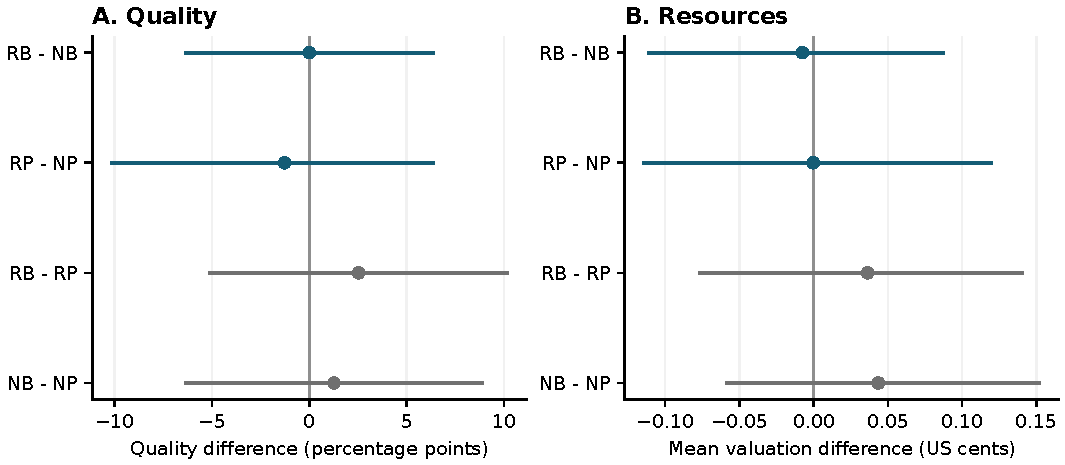
\includegraphics[width=\linewidth]{figures/segregation80/effects.pdf}
\caption{Independent experiment: paired quality differences (percentage points) and API-equivalent valuation differences (US cents per candidate), with descriptive 95\% task-bootstrap intervals. The first two contrasts form the primary quality-test family; the layout contrasts are descriptive. RB/NB denote role/neutral headings, RP/NP role/neutral prose.}\label{fig:seg80-effects}
\end{figure}

The additional wording-and-layout experiment therefore does not convincingly reproduce the primary series' 18.45\% lower valuation for the single-call role condition. This comparison across batches is descriptive: task sample, precise instructions, execution time, environment and deadline differ, and no formal between-study heterogeneity test is claimed. The new estimates limit generalization of the earlier resource finding to role names alone. They do not invalidate the recorded primary observations, prove zero effect, or test the three-call topology. The two prospective analyses remain separate.
